\section{En beskrivning av fastigheten på Walleriusgatan och dess konstruktion}
\label{subsec:thehouse}
% Johanneberg 7:8

% Hur tänkte de när de byggde och renoverade huset?
% Vad ville de uppnå och vilka regler och normer hade man att hålla sig till?

% Att huset är byggt så här vad betyder det för hur huset påverkas och hur huset är att bo i?

% Det är så här stort och har så här många rum, så här högt i tak o.s.v. 

Projektets uppdragsgivare har hand om energisystemet i en fastighet i Johanneberg,
Göteborg som kan ses i bild~\ref{fig:thehouse:house}. Figur~\ref{fig:thehouse:map}
visar fastighetens geografiska orientering.
Det är den fastighet som varit i fokus för det här arbetet. Byggnaden uppfördes 1935\cite{ritningar_urspr}
och sedan kom det att dröja ända till 1988 innan den första större ombyggnationen gjordes.
Då gjordes två lägenheter om till kontor, stammar byttes och vinden byggdes om till lägenheter.
Både taket, burspråken på södersidan och den norra fasaden tilläggsisolerades.
I samband med detta installerades också nya värme- och ventialtionssystem och alla
fönster byttes och tätades med expanderskum. Den främsta skillnaden för de boende
blev minskat drag vid blåst och bättre ventilation.  Med det nya ventilationssystemet
byts luften helt och hållet varannan timme och den friska luften värmeväxlas också med den gamla för att minska energiförlusterna. Enligt Peter Särneö\cite{petersarneo}
förbrukar fastigheten idag mindre energi än ett nybyggt hus.

\begin{figure}
\centering
\includegraphics[width=130mm,height=87mm]{images/house.eps}
\caption{Fastigheten Johanneberg 7:8 på Walleriusgatan i Göteborg.}
\label{fig:thehouse:house}
\end{figure}

\begin{figure}
\centering
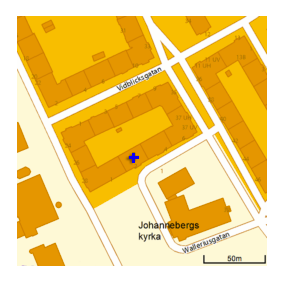
\includegraphics[width=1.67in,height=1.67in]{images/map.eps}
\caption{Kartbild över fastigheten, som är markerad med \textbf{\color{blue}+}. Fasaden som vätter mot söder är vinklad $\unit[32]{^\circ}$ från
ost-västlig riktning.}
\label{fig:thehouse:map}
\end{figure}

Fastigheten har idag 13 lägenheter och en kontorslokal på $\unit[225]{m^2}$. De utgör tillsammans $\unit[1450]{m^2}$ fördelat på sju våningar. Utöver detta finns det gemensamma utrymmen, trapphus, förråd och apparatrum i den nedre källaren och Peter Särneö\cite{petersarneo} bedömer att den totala ytan är cirka $\unit[2000]{m^2}$. Sedan ett tag tillbaka har även en väderstation och en solintensitetsmätare installerats, se avsnitt~\ref{subsec_weathertransmitter}, i förhoppningen att de ska kunna utnyttjas för att förbättra fastighetens klimat ytterligare- Det är det här projektets uppgift att undersöka hur det ska kunna genomföras.

För att göra beräkningar av värmeflödet genom väggarna vid olika väderförhållanden har U-värdet varit ett centralt begrepp. De beräknas utifrån materialets tjocklek och värmeledningsförmåga, se avsnitt~\ref{sec:heatconduction}. U-värdet är ett mått på väggens förmåga att släppa igenom värme och mäts i $\unit{W~m^{-2}~K^{-1}}$. För en vägg med flera lager summeras U-värden på samma sätt som resistansen parallellkopplade resistorer:
\begin{equation}
\label{eq:uvalue}
\frac{1}{U_{tot}}= (\frac{1}{U_1}+...+\frac{1}{U_n}).
\end{equation}
Väggarnas olika U-värden presenteras i tabell \ref{tbl:uvalue}.

\begin{table}[hbtp]
\centering
\caption{Areor och U-värden för fastighetens klimatsköld.}
\label{tbl:uvalue}

\begin{tabular}
{|l|r|r|}
\hline
\textbf{Del} & \textbf{Area $[\unit{m^2}]$} & \parbox[c][1.2cm][c]{2 cm}{\textbf{U-värde\\$[\unit{W~m^{-2}~K^{-1}}]$}} \\
\hline
Söderväggen &  151 & 1,186 \\ 
Västerväggen & 61 & 1,186 \\
Norrväggen & 290 & 0,279 \\
Burspråket & 47 & 0,393 \\
Taket & 257 & 0,171 \\
\hline
Fönster, söder & 109 & 1,0 \\
Fönster, norr & 89 & 1,0 \\
Fönster, tak & 8 & 1,0 \\
\hline
\textbf{Totalt} & \textbf{1012} & \textbf{0,6}\\
\hline
\end{tabular}
\end{table}

Det genomsnittliga U-värdet för fastigheten, grunden borträknad, är $\unit[0,6]{W~m^{-2}~K^{-1}}$

% De olika gränsytornas material och uppbyggnad.
\subsection{Väggarna}
\label{subsec:walls}

\begin{figure}[hpbt]
\centering
\subfloat[
	\label{fig:sodervagg}Söderväggen tillika västerväggen, utifrån och in från vänster till höger. Alla mått är i mm.
	]{
	\parbox[c]{7cm}{
	\centering
	\raisebox{0.5cm}{
		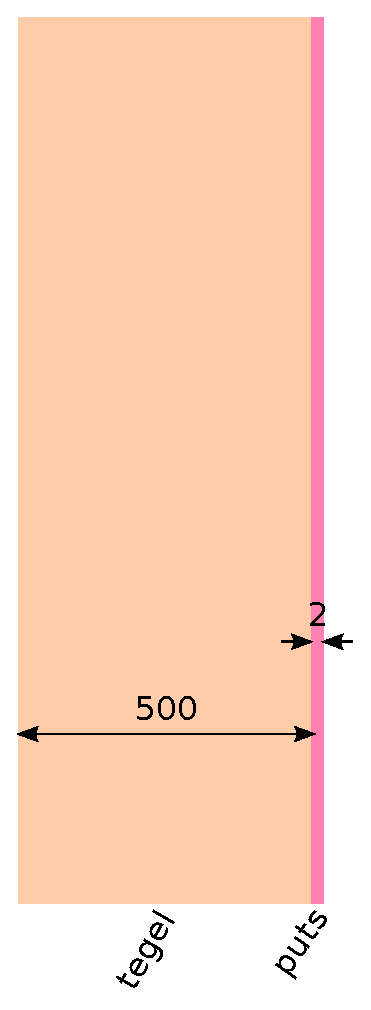
\includegraphics[width=2.21cm]{images/sodervagg.eps}
	}
	}
}
\subfloat[\label{fig:norrvagg}Norrväggen, utifrån och in från vänster till höger. Alla mått är i mm.]{
	\parbox[c]{7cm}{
	\centering
	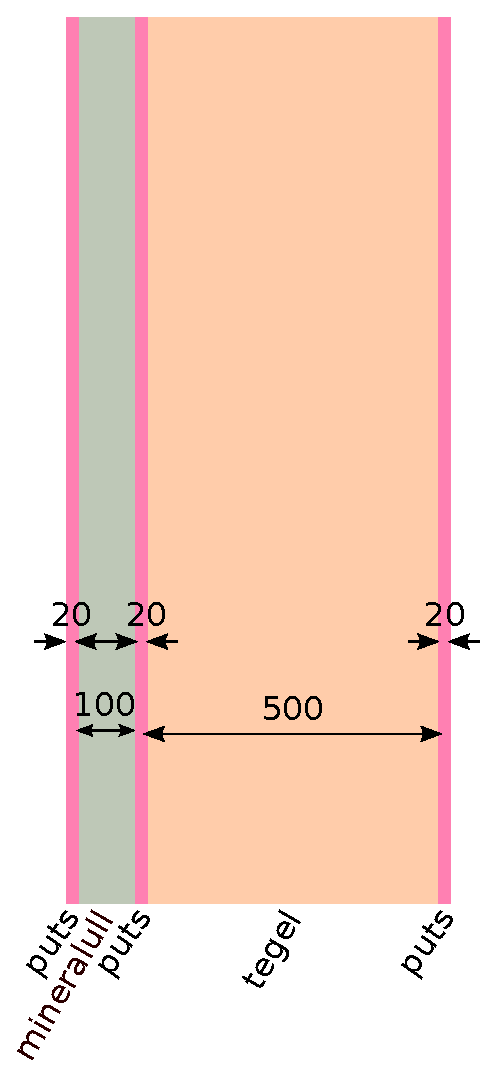
\includegraphics[width=3cm]{images/norrvagg.eps}
}
}

\caption{\label{fig:thewalls} Väggarnas konstruktion.}
\end{figure}

Ytterväggarna bestod ursprungligen av \unit[0,5]{m} tegel, klätt med ett centimetertjockt lager av puts på insidan,
se figur~\ref{fig:sodervagg}. Norrväggen, som tilläggsisolerades i samband med renoveringen 1988, har dessutom puts och ett decimetertjockt lager mineralull följt av ett lager puts utanpå tegelväggen,
se figur~\ref{fig:norrvagg}.\cite{kandidatarbete2010}\cite{petersarneo}. Då värmeledningsförmågan hos tegel är
$\unit[0,593]{W~m^{-1}~K^{-1}}$ och den för mineralull är $\unit[0,037]{W~m^{-1}~K^{-1}}$
fås att den isolerade norrväggen har ett U-värde på $\unit[0,279]{W~m^{-2}~K^{-1}}$
medan den oisolerade söderväggens U-värde är $\unit[1,186]{W~m^{-2}~K^{-1}}$.

\begin{figure}[hpbt]
\centering
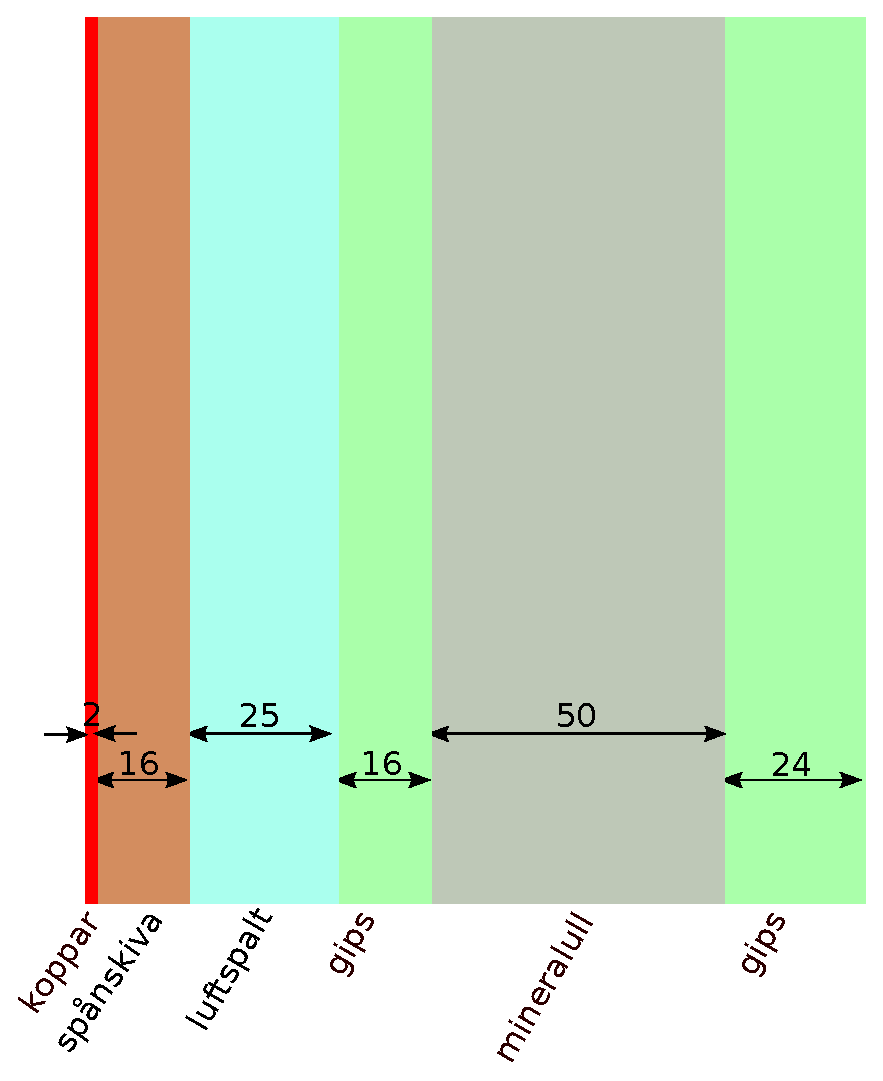
\includegraphics[width=6cm]{images/bursprak.eps}
\caption{\label{fig:bursprak}{Burspråket på söderväggen, utifrån och in från vänster till höger. Alla mått är i mm.}}
\end{figure}

Fastigheten ligger mellan två andra byggnader i liknande stil. Den till öster är lika hög som fastigheten medan den i väster är något lägre. Fastighetens yttervägg i väster är inte tilläggsisolerad och har samma konstruktion som söderväggen, se figur~\ref{fig:sodervagg}.

På söderväggen finns ett kopparklätt burspråk. Kopparn sitter direkt på en cementbunden spånskiva som följs av en luftspalt. Väggen innanför består av gips, isolerade mineralull och sedan mer gips, se figur~\ref{fig:bursprak}.\cite{kandidatarbete2010} Burspråkets U-värde är $\unit[0,393]{W~m^{-2}~K^{-1}}$.

\subsection{Taket}
Även taket lades om i samband med den stora renoveringen. Därefter bestod det av taktegel på underlagspapp ytterst, följt av gips, isolerande mineralull och innerst ytterligare ett lager gips, se figur~\ref{fig:taket}.\cite{kandidatarbete2010}. U-värdet för taket är $\unit[0,171]{W~m^{-2}~K^{-1}}$.

Direkt under taket finns en lägenhet som givetvis är uppvärmd. Precis under taknocken finns ett mindre utrymme, se figur~\ref{fig:attic}, som bland annat kan användas för kablar.

\begin{figure}[hpbt]
\centering
\subfloat[
	\label{fig:taket}Takets konstruktion. Alla mått är i mm.
	]{
	\parbox[c]{7cm}{
	\centering
		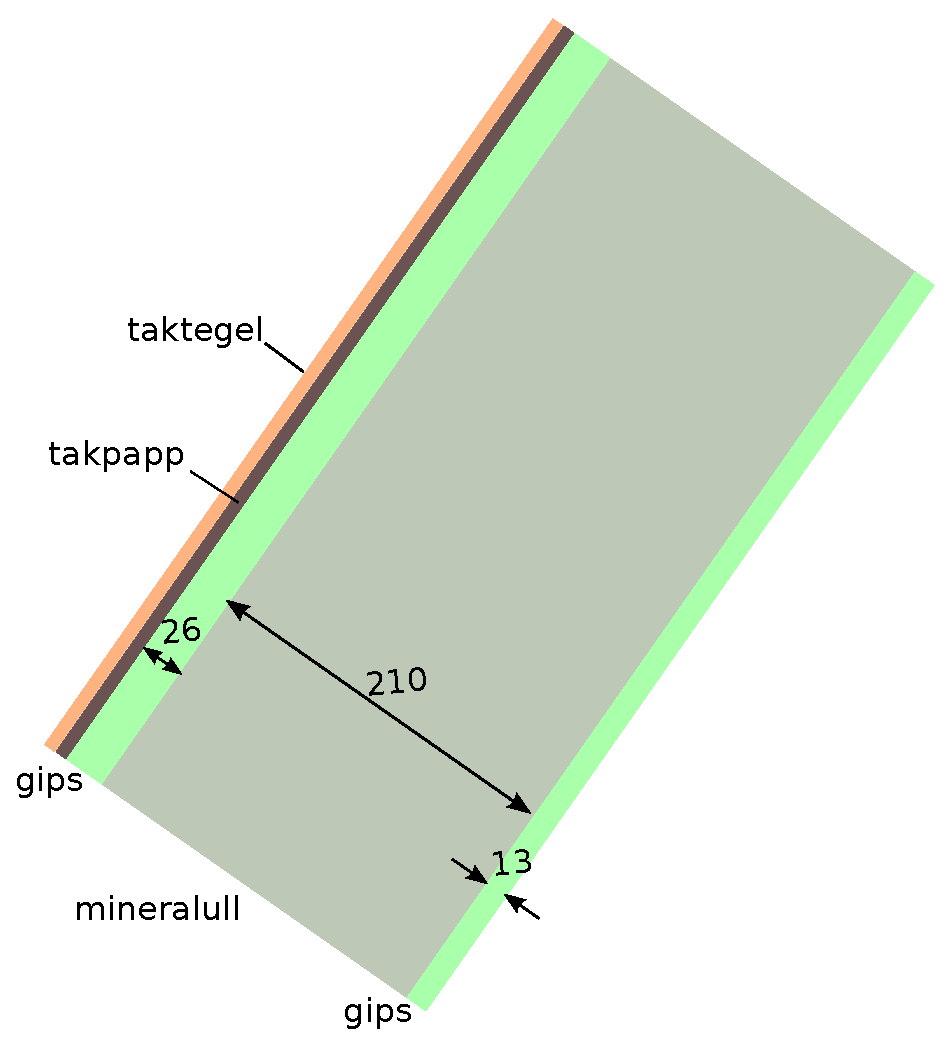
\includegraphics[width=5cm]{images/taket.eps}
	}
}
\subfloat[\label{fig:attic}Fastighetens översta våning, från ritningen\cite{ritningar_urspr}.]{
	\parbox[c]{7cm}{
		\raisebox{-4.5cm}{
			\centering
			\includegraphics[width=5cm]{images/attic.eps}
			\begin{minipage}[c][2.0cm]{3cm}{~}
			\end{minipage}
		}
	}
}
\caption{\label{fig:roof_attic} Takets och vindens respektive konstruktioner.}
\end{figure}


\subsection{Fönstren}

Byggnadens fönster sattes in 1988 och är av treglastyp utan ytbeläggningar. De två yttersta rutorna är isolerglas, det vill säga de två rutorna avgränsar ett hermetiskt tillslutet utrymme, och den inneslutna volymen är fylld med argon för att minska värmeledningsförmågan. Totalt har fönstren ett U-värde på ungefär $\unit[1]{W~m^{-2}~K^{-1}}$.

\subsection{Grunden}

Huset är byggt på ett berg som sluttar kraftigt. I östra delen av fastigheten ligger huset direkt på berget med endast ett lager av makadam emellan\cite{petersarneo}. I västra halvan har huset en undre källare där apparat- och fläktrummen finns. Där är det betydligt större avstånd ned till berget, uppskattningsvis ett par meter. % Mer exakt? Källa?

\subsection{Uppvärmning och ventilation}
Idag värms huset av bergvärme från tre bergvärmepumpar. För att minska energiåtgången har ett flertal värmeväxlare installerats och värmen från all frånluft återanvänds i möjligaste mån. Peter Särneö gör bedömningen att detta är ett tämligen effektivt energiförsörjningssytem. Det är inte här de stora energivinsterna kan göras i den här fastigheten. Varifrån energin för uppvärmning av fastigheten kommer är inte heller något som behandlas inom det här arbetet.
